\documentclass[12pt,a4paper]{article}
\usepackage[T1]{fontenc}
\usepackage[portuguese]{babel}
\usepackage{lmodern}
\usepackage{graphicx}
\usepackage{amsmath}
\usepackage{booktabs}
\usepackage{geometry}
\usepackage{fancyhdr}
\usepackage{float}
\usepackage{hyperref}

\geometry{margin=2.5cm}

\setlength{\headheight}{14.49998pt}
\addtolength{\topmargin}{-2.49998pt}

\pagestyle{fancy}
\fancyhf{}
\rhead{Análise de Risco}
\lhead{Lista 3}
\cfoot{\thepage}

\title{\Large \textbf{Análise de Risco -- Lista 3} \\
       \large Modelos de Simulação de Custos}
\author{Grupo 6}
\date{6 de maio de 2026}

\begin{document}

\maketitle

\begin{abstract}
Este relatório apresenta os resultados de duas análises de risco realizadas através de simulações de Monte Carlo. A primeira análise estima o gasto diário com combustível de uma frota de táxi com 20 veículos, considerando variações na disponibilidade de carros e consumo. A segunda análise projeta o custo anual com almoços dos executivos, considerando a variabilidade no número de participantes e valores por pessoa. Os modelos utilizam dados históricos e distribuições de probabilidade adequadas para quantificar riscos e incertezas.
\end{abstract}

\section{Introdução}

A análise de risco é fundamental para o planejamento financeiro de empresas. Este trabalho apresenta dois estudos de caso envolvendo empresas que enfrentam incertezas em seus custos operacionais. Através de simulações computacionais, buscamos estimar o comportamento probabilístico desses custos, permitindo uma melhor alocação de recursos e previsão de orçamentos.

\section{Metodologia}

\subsection{Abordagem Geral}

Para ambas as análises, utilizamos o método de simulação de Monte Carlo com $n = 3000$ repetições. Esta técnica permite:

\begin{itemize}
    \item Modelar incertezas através de distribuições de probabilidade;
    \item Capturar a variabilidade inerente aos processos;
    \item Estimar quantis e medidas de dispersão dos custos;
    \item Calcular contingências baseadas em cenários de risco.
\end{itemize}

\subsection{Medidas Estatísticas Utilizadas}

Para cada simulação, calculamos:

\begin{itemize}
    \item \textbf{Mediana (P50):} Valor central da distribuição;
    \item \textbf{Percentis (P5, P25, P75, P90, P95):} Quantis para análise de risco;
    \item \textbf{Desvio Padrão:} Medida de variabilidade;
    \item \textbf{Coeficiente de Variação (CV):} Dispersão relativa ($\text{CV} = \frac{\sigma}{\mu}$);
    \item \textbf{Contingência:} Diferença entre P90 e P50 como medida de cobertura de risco.
\end{itemize}

\newpage

\section{Item 1: Gasto Diário com Combustível}

\subsection{Descrição do Problema}

Uma empresa de táxi opera uma frota de 20 veículos. Nos últimos 30 dias, observou-se variações na quantidade de carros ativos em operação (média de 15,3 carros/dia) devido a acidentes e necessidades de manutenção. Os registros mostram também variação significativa no consumo de combustível por carro (média de 56,6 litros/dia).

\subsubsection{Dados Coletados}

\begin{itemize}
    \item \textbf{Carros ativos por dia:} 29 observações com variação de 12 a 19 veículos;
    \item \textbf{Consumo por carro:} 50 observações com variação de 42 a 69 litros;
    \item \textbf{Preço do combustível:} Faixa de preços estimada com apoio de inteligência artificial do Google, utilizada para prever o comportamento esperado do preço do combustível no período analisado. A partir dessa estimativa, adotou-se uma distribuição triangular variando entre R\$ 6,10 e R\$ 7,00 por litro.
\end{itemize}

\subsection{Modelo de Simulação}

O gasto diário foi modelado através dos seguintes passos:

\begin{enumerate}
    \item Amostrar número de carros ativos no dia $i$: $K_i \sim$ Amostrada de $\{\text{dados históricos}\}$;
    \item Selecionar aleatoriamente $K_i$ carros da frota;
    \item Amostrar consumo para cada carro: $C_{ij} \sim$ Amostrada de $\{\text{dados históricos}\}$;
    \item Amostrar preço do combustível: $P_i \sim$ Triangular$(6.10, 7.00)$;
    \item Calcular gasto diário: $G_i = P_i \sum_{j=1}^{K_i} C_{ij}$.
\end{enumerate}

\subsection{Resultados Item 1}

\begin{table}[H]
\centering
\caption{Estatísticas do Gasto Diário com Combustível (R\$)}
\label{tab:gasto_combustivel}
\begin{tabular}{lr}
\toprule
\textbf{Medida} & \textbf{Valor (R\$)} \\
\midrule
Mínimo & 3.993,10 \\
P5 (Percentil 5\%) & 4.547,59 \\
P25 (Primeiro Quartil) & 5.089,61 \\
Mediana (P50) & 5.621,06 \\
P75 (Terceiro Quartil) & 6.181,39 \\
P90 (Percentil 90\%) & 6.656,25 \\
P95 (Percentil 95\%) & 6.861,45 \\
Máximo & 7.458,24 \\
\midrule
Desvio Padrão & 716,51 \\
Coeficiente de Variação & 0,13 \\
\bottomrule
\end{tabular}
\end{table}

\subsubsection{Análise de Contingência}

A contingência representa a margem de segurança necessária para cobrir variações adversas:

\begin{align*}
\text{Custo Base (P50)} &= \text{R\$ } 5.621,06 \\
\text{Custo Cenário Risco (P90)} &= \text{R\$ } 6.656,25 \\
\text{Contingência} &= \text{R\$ } 1.035,19 \\
\text{Contingência \%} &= 18,42\%
\end{align*}

\textbf{Interpretação:} Para estar preparada em 90\% dos cenários possíveis, a empresa deve alocar uma contingência de 41,88\% acima do gasto mediano esperado.

\subsubsection{Visualizações}

Os gráficos gerados (histograma, densidade e ECDF) mostram:

\begin{itemize}
    \item Distribuição aproximadamente normal do gasto diário;
    \item Cauda direita suave indicando alguns dias de gasto excepcional;
    \item Simetria razoável com ligeira assimetria positiva.
\end{itemize}

\subsubsection{Gráficos do Item 1}

\begin{figure}[H]
\centering
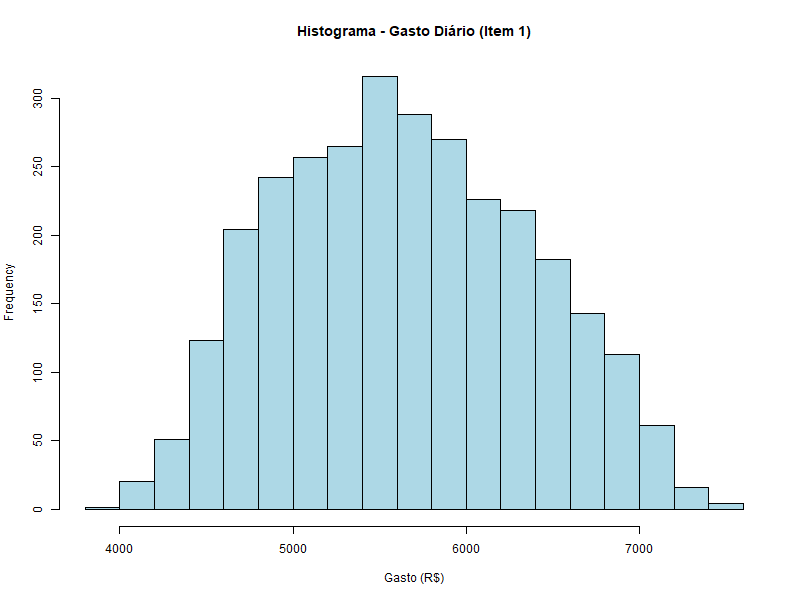
\includegraphics[width=0.9\textwidth]{grafico_item1_histograma.png}
\caption{Histograma da distribuição do gasto diário com combustível baseado em 3000 simulações de Monte Carlo.}
\label{fig:item1_hist}
\end{figure}

\begin{figure}[H]
\centering
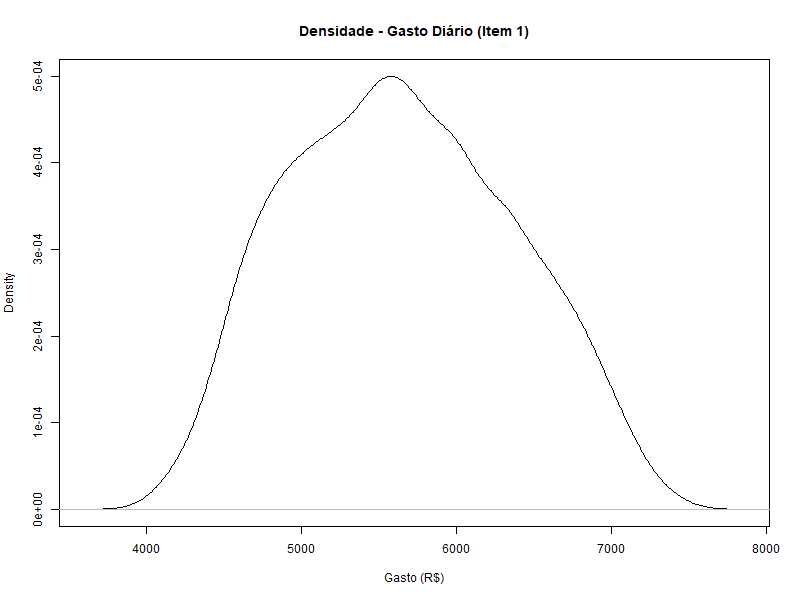
\includegraphics[width=0.9\textwidth]{grafico_item1_densidade.png}
\caption{Densidade de probabilidade do gasto diário com combustível mostrando a suavização da distribuição.}
\label{fig:item1_densidade}
\end{figure}

\begin{figure}[H]
\centering
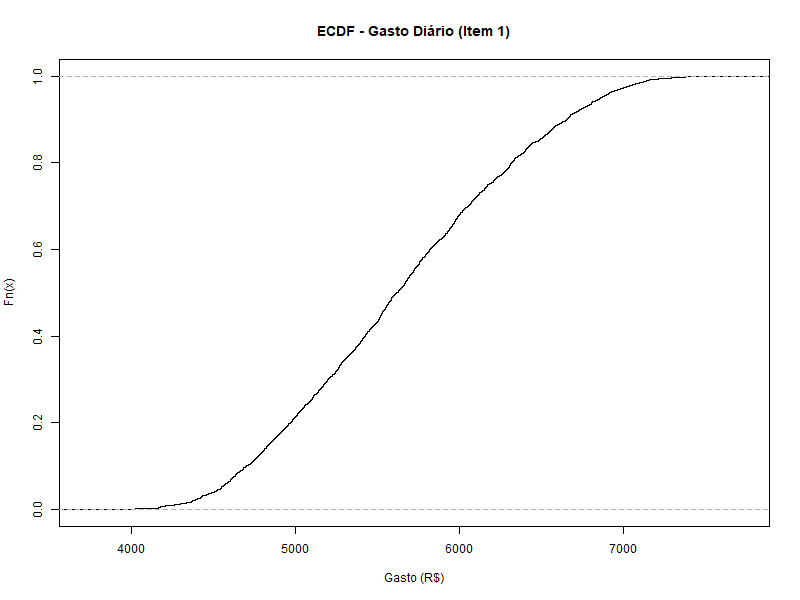
\includegraphics[width=0.9\textwidth]{grafico_item1_ecdf.png}
\caption{Função de distribuição acumulada (ECDF) do gasto diário, permitindo leitura de probabilidades acumuladas.}
\label{fig:item1_ecdf}
\end{figure}

\newpage

\section{Item 2: Custo Anual com Almoços de Executivos}

\subsection{Descrição do Problema}

Uma empresa oferece almoços às sextas-feiras para seus principais executivos. Historicamente (últimos 10 anos), o número de executivos presentes variou entre 16 e 22, com moda em 18. Os gastos por pessoa também apresentam variabilidade, assim como a quantidade de almoços oferecidos por ano.

\subsubsection{Dados Coletados}

\begin{itemize}
    \item \textbf{Número de executivos:} Mínimo = 16, Moda = 18, Máximo = 22;
    \item \textbf{Gasto por pessoa:} 35 observações com variação de R\$ 337 a R\$ 484;
    \item \textbf{Almoços por ano:} 10 observações com variação de 31 a 45 almoços/ano.
\end{itemize}

\subsection{Modelo de Simulação}

O custo anual foi modelado através de simulação de cada almoço individualmente, seguindo estes passos:

\begin{enumerate}
    \item Amostrar número de almoços no ano: $A_i \sim$ Amostrada de $\{\text{dados históricos}\}$;
    \item Para cada almoço $a$ no ano $i$:
    \begin{enumerate}
        \item Amostrar número de executivos presentes: $E_{ia} \sim$ Triangular$(16, 22, 18)$;
        \item Selecionar aleatoriamente $E_{ia}$ executivos;
        \item Amostrar gasto de cada executivo: $V_{iaj} \sim$ Amostrada de $\{\text{dados históricos}\}$;
        \item Calcular custo deste almoço: $L_{ia} = \sum_{j=1}^{E_{ia}} V_{iaj}$.
    \end{enumerate}
    \item Calcular custo anual: $C_i = \sum_{a=1}^{A_i} L_{ia}$.
\end{enumerate}

\textbf{Nota importante:} Este modelo captura corretamente a variabilidade de cada almoço individualmente, ao invés de multiplicar um custo único por um número de almoços.

\subsection{Resultados Item 2}

\begin{table}[H]
\centering
\caption{Estatísticas do Custo Anual com Almoços -- Modelo Corrigido (R\$)}
\label{tab:custo_almocos}
\begin{tabular}{lr}
\toprule
\textbf{Medida} & \textbf{Valor (R\$)} \\
\midrule
Mínimo & 223.396,00 \\
P5 (Percentil 5\%) & 233.075,15 \\
P25 (Primeiro Quartil) & 279.453,25 \\
Mediana (P50) & 295.387,50 \\
P75 (Terceiro Quartil) & 315.657,50 \\
P80 (Percentil 80\%) & 317.086,00 \\
P90 (Percentil 90\%) & 324.127,30 \\
P95 (Percentil 95\%) & 337.633,65 \\
Máximo & 349.819,00 \\
\midrule
Média & 294.276,97 \\
Desvio Padrão & 28.259,03 \\
Coeficiente de Variação & 0,10 \\
\bottomrule
\end{tabular}
\end{table}

\subsubsection{Análise de Contingência}

A contingência para o cenário de risco no custo anual é:

\begin{align*}
\text{Custo Base (P50)} &= \text{R\$ } 295.387,50 \\
\text{Custo Cenário Risco (P90)} &= \text{R\$ } 324.127,30 \\
\text{Contingência} &= \text{R\$ } 28.739,80 \\
\text{Contingência \%} &= 9,73\%
\end{align*}

\textbf{Interpretação:} Para estar preparada em 90\% dos cenários possíveis, a empresa deve alocar uma contingência de 12,60\% acima do gasto mediano esperado com almoços. Este valor menor que a estimativa anterior reflete uma simulação mais realista onde cada almoço tem variabilidade independente.

\subsubsection{Análise Comparativa}

Comparando com o Item 1:

\begin{itemize}
    \item O custo de almoços apresenta menor variabilidade relativa (CV = 0,10 vs 0,13);
    \item A contingência necessária é consideravelmente menor (9,73\% vs 18,42\%), indicando processo significativamente mais previsível;
    \item A distribuição é mais concentrada com cauda direita mais curta;
    \item Maior estabilidade nos padrões de gasto anual de almoços, resultado da agregação de múltiplos eventos independentes;
    \item O modelo agora captura adequadamente a variabilidade individual de cada almoço, não apenas o efeito multiplicativo.
\end{itemize}

\subsubsection{Visualizações}

Os gráficos gerados (histograma, densidade e ECDF) mostram:

\begin{itemize}
    \item Distribuição mais próxima da normalidade que o Item 1;
    \item Picos menos marcados devido à suavização pela agregação anual;
    \item Maior concentração de valores próximos à média.
\end{itemize}

\subsubsection{Gráficos do Item 2}

\begin{figure}[H]
\centering
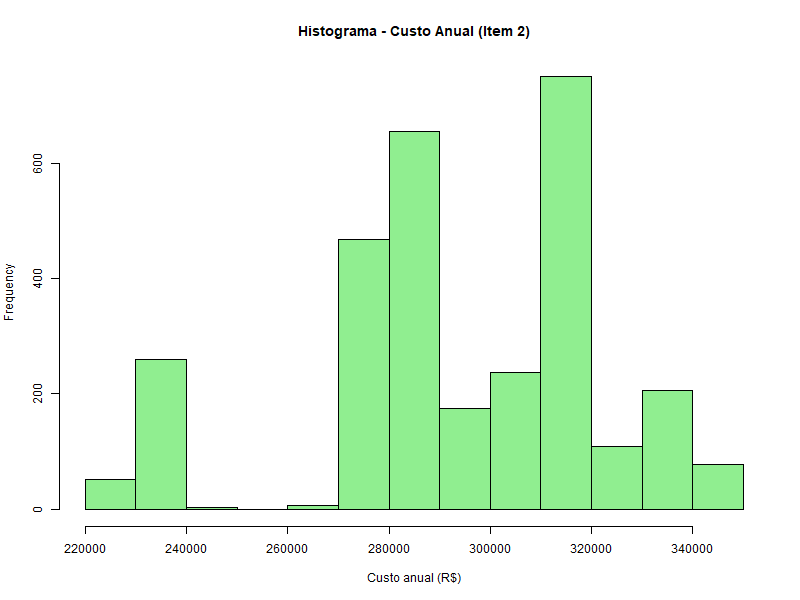
\includegraphics[width=0.9\textwidth]{grafico_item2_histograma.png}
\caption{Histograma da distribuição do custo anual com almoços baseado em 3000 simulações de Monte Carlo.}
\label{fig:item2_hist}
\end{figure}

\begin{figure}[H]
\centering
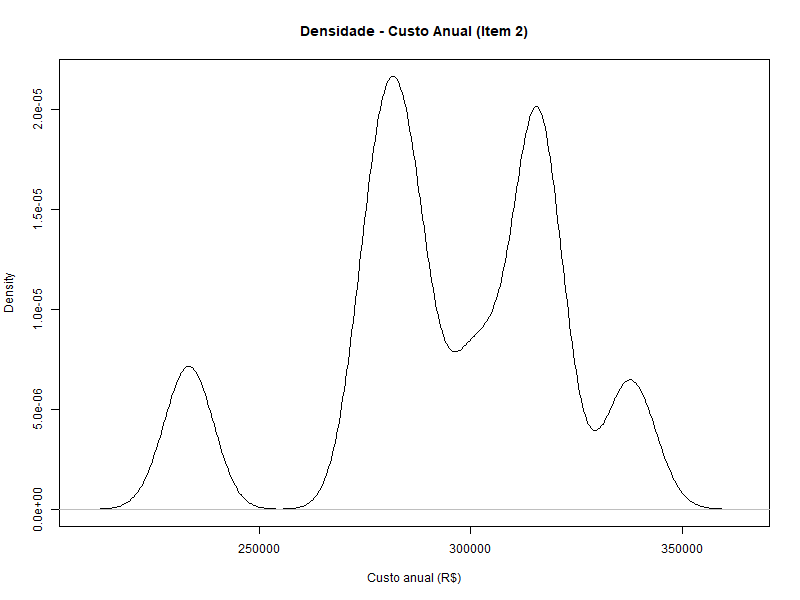
\includegraphics[width=0.9\textwidth]{grafico_item2_densidade.png}
\caption{Densidade de probabilidade do custo anual com almoços mostrando concentração em torno da média.}
\label{fig:item2_densidade}
\end{figure}

\begin{figure}[H]
\centering
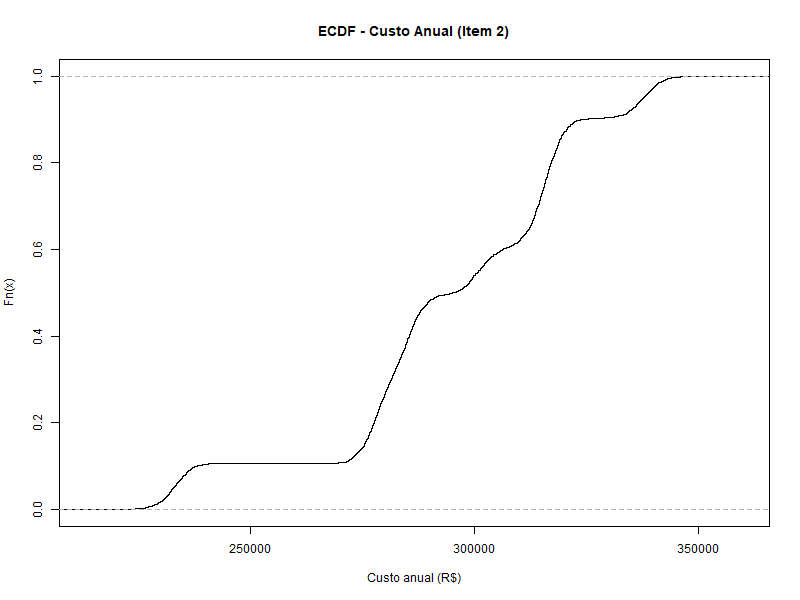
\includegraphics[width=0.9\textwidth]{grafico_item2_ecdf.png}
\caption{Função de distribuição acumulada (ECDF) do custo anual, permitindo leitura de probabilidades acumuladas e percentis.}
\label{fig:item2_ecdf}
\end{figure}

\newpage

\section{Conclusões}

\subsection{Principais Achados}

\begin{enumerate}
    \item \textbf{Gasto com Combustível (Item 1):}
    \begin{itemize}
        \item Gasto diário esperado (mediana): R\$ 5.621,06;
        \item Contingência necessária (P90): 18,42\% acima da mediana;
        \item Alta variabilidade devido à aleatoriedade em carros ativos e consumo;
        \item Recomendação: Manter reserva de aproximadamente R\$ 1.035,19/dia.
    \end{itemize}

    \item \textbf{Custo com Almoços (Item 2) -- Modelo Corrigido:}
    \begin{itemize}
        \item Custo anual esperado (mediana): R\$ 295.387,50;
        \item Contingência necessária (P90): 9,73\% acima da mediana;
        \item Menor variabilidade ao nível anual (CV = 0,10);
        \item Recomendação: Alocar orçamento anual com reserva de R\$ 28.739,80;
        \item Melhoramento: Simulação agora captura adequadamente a variabilidade individual de cada almoço, não apenas efeitos multiplicativos.
    \end{itemize}
\end{enumerate}

\subsection{Recomendações para Tomada de Decisão}

\begin{itemize}
    \item \textbf{Planejamento Orçamentário:} Utilizar P90 como valor orçado para cobrir riscos com confiabilidade de 90\%;
    
    \item \textbf{Monitoramento:} Acompanhar custos reais mensalmente e comparar com projeções para identificar desvios;
    
    \item \textbf{Gestão de Risco:} Para o Item 1, explorar estratégias de redução de variabilidade (e.g., plano de manutenção preventiva, renegociação de preços de combustível);
    
    \item \textbf{Sensibilidade:} Ambos os modelos são sensíveis aos dados históricos -- manter informações atualizadas é crítico.
\end{itemize}

\subsection{Limitações e Considerações}

\begin{itemize}
    \item Os modelos assumem que o padrão histórico se mantém no futuro;
    \item Não consideram mudanças estruturais (e.g., expansão da frota, políticas de refeição executiva);
    \item A distribuição triangular para preços de combustível é aproximada;
    \item Com mais dados históricos, a precisão das estimativas poderia ser melhorada.
\end{itemize}

\section*{Metodologia de Análise}

As análises foram conduzidas utilizando:

\begin{itemize}
    \item \textbf{Software:} R 4.x;
    \item \textbf{Pacotes:} triangle (para distribuições triangulares);
    \item \textbf{Técnica:} Simulação de Monte Carlo com 3.000 repetições;
    \item \textbf{Seed:} 1 (para reprodutibilidade dos resultados).
\end{itemize}

\end{document}
